\def \withcache{1}
\documentclass{../cours}
\usepackage{hyperref}
\title{Cours 3 : Récursivité}


\begin{document}
\maketitle
 
\section{Définition et premiers exemples}

\subsection{Rappel : la pile d'exécution}

Au cours de l'exécution d'un programme les variables sont stockées dans la mémoire sous forme d'une \textbf{pile}. A chaque appel de fonction, un espace mémoire est réservé pour les variables de la fonction.

\begin{Example}.

\lstset{numbers=left}
\begin{lstlisting}
Fonction Fonction1(entier a):
	Entier c <- a+1    
    Retourner c
    
    
Fonction Fonction2(entier b):
    Retourner Fonction1(b+1)

Fonction Principale():
	Entier a <- Fonction2(3)
	...
\end{lstlisting}

\begin{tabular}{ccc}

\begin{tabular}{|l|}
\\
\hline
\\
\hline
\\
\hline
\\
\hline
\\
\hline
\\
\hline
\\
\hline
{\tt a} : ?~~~~~~~~~~~~~~~~
\\
\hline
\\
\end{tabular}

&

\begin{tabular}{|l|}
\\
\hline
\\
\hline
\\
\hline
\\
\hline
{\tt b} : 3\\
\hline
Retour : ?\\
\hline
Info {\tt Fonction2}: ...  \\
\hline
{\tt a} : ?~~~~
\\
\hline
\\
\end{tabular}

&

\begin{tabular}{|l|}
a : 4
\\ \hline
c: ?
\\ \hline
Retour : ?
\\ \hline
Info {\tt Fonction1}: ...\\
\hline
{\tt b} : 3\\
\hline
Retour : ?\\
\hline
Info {\tt Fonction2}: ...  \\
\hline
{\tt a} : ?~~~~
\\
\hline
\\
\end{tabular}

\\
Début de la fonction principale
&
Appel de {\tt Fonction2} (ligne 10)
&
Appel de {\tt Fonction1} (ligne 7)
\\

\\

\begin{tabular}{|l|}
a : 4
\\ \hline
c: 5
\\ \hline
Retour : 5
\\ \hline
Info {\tt Fonction1}: ...\\
\hline
{\tt b} : 3\\
\hline
Retour : ?\\
\hline
Info {\tt Fonction2}: ...  \\
\hline
{\tt a} : ?~~~~
\\
\hline
\\
\end{tabular}

&

\begin{tabular}{|l|}

\\ \hline

\\ \hline

\\ \hline
\\
\hline
{\tt b} : 3\\
\hline
Retour : 5\\
\hline
Info {\tt Fonction2}: ...  \\
\hline
{\tt a} : ?~~~~
\\
\hline
\\
\end{tabular}

&


\begin{tabular}{|l|}

\\ \hline

\\ \hline

\\ \hline
\\
\hline
\\
\hline
\\
\hline
\\
\hline
{\tt a} : 5~~~~~~~~~~~~~~~~
\\
\hline
\\
\end{tabular}

\\
Fin d'appel {\tt Fonction1} (ligne 3)
&
Fin d'appel {\tt Fonction2} (ligne 7)
& 
Retour Fonction {\tt Pincipale}
\end{tabular}
\end{Example}

En particulier, rien n'empêche une fonction de s'appeler elle-même.

\begin{Example}
Que se passe-t-il au niveau de la pile dans l'exemple suivant ?

\begin{lstlisting}
Fonction Fonction1(entier a):
    Fonction1(a)
    
Fonction Principale():
    Fonction1(3)
\end{lstlisting}
\end{Example}

\subsection{Définition}

\begin{Definition}
Un algorithme \emph{récursif} est un algorithme qui fait appel à lui même. Lorsqu'un algorithme n'est pas récursif, on dit qu'il est \emph{itératif}.
\end{Definition}

Pour éviter une boucle infinie, il faudra impérativement définir \textbf{une condition d'arrêt}.

\begin{Example}
Le calcul de $n!$. Tout d'abord la version itérative

\begin{lstlisting}
Fonction factorielle(entier n):
    Entier r <- 1
    Pour i allant de 1 à n:
        r <- r * i
    Retourner r
\end{lstlisting}

La version récursive se base sur le principe suivant :

\begin{equation}
n! = \begin{cases}
1 & \text{si } n = 0 \\
n \times (n-1)! & \text{sinon}
\end{cases},
\end{equation}
que l'on peut traduire sous forme d'algorithme.

\begin{lstlisting}
Fonction factorielle(entier n):
    Si n = 0:
        Retourner 1
    Retourner n * factoriel(n-1)
\end{lstlisting}
\end{Example}

\subsection{Comment définir une fonction récursive}

Le principe d'une fonction récursive est assez similaire à la notion de \textbf{récurrence} mathématique. On ne cherche pas à calculer le problème dans son ensemble mais simplement à le définir en fonction d'un problème de taille plus petite. Tout comme en mathématique le fait de prouver l'état initial et une seule étape permet de prouver la propriété, dans un algorithme, le fait de calculer l'état initial et une étape permet de calculer n'importe quelle valeur. 

Un algorithme récursif s'écrira toujours de cette façon :

\begin{lstlisting}
Input : des paramètres
Processus:
    Si les paramètres correspondent à la condition d'arret (cas simple):
        Actions cas d'arret
    Sinon
        Appel(s) récursifs sur de nouveaux paramètres
\end{lstlisting}

Pour être sûr que l'algorithme termine, les nouveaux paramètres doivent se rapprocher de la condition d'arrêt.

\begin{Example}
Les tours de Hanoi

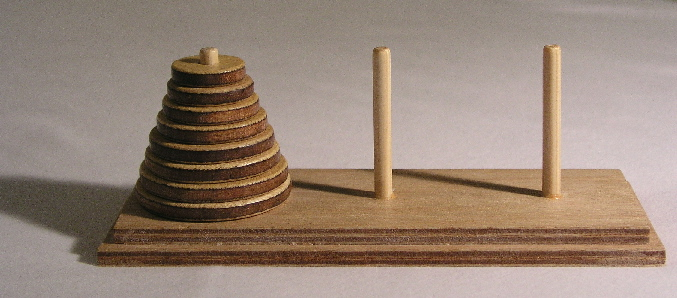
\includegraphics[scale=0.5]{hanoi.jpg}

Problème : on possède trois pics sur lesquels sont empilés des disques de tailles décroissantes (tous sur le premier pic). On souhaite déplacer la pile sur le second pic en suivant les règles suivantes:
\begin{itemize}
\item on ne peut déplacer qu'un seul disque à la fois, celui du haut de la pile,
\item on ne peut poser un disque que sur un disque plus grand.
\end{itemize}

On suppose donc que l'on dispose d'une seule action possible :
\begin{lstlisting}
Fonction Déplacer
Input : 
    - le pic de départ
    - le pic d'arrivée
Processus :
    Si départ n'est pas vide:
        D <- disque retiré au sommet de départ
    Sinon:
        Erreur "Départ est vide"
    Si D < disque au sommet d'arrivée:
        Poser D au sommet d'arrivée
    Sinon:
        Erreur "Action impossible"
\end{lstlisting}
\textbf{Comment résoudre ce problème ?}

Pour résoudre un problème de façon récursive, il faut répondre à plusieurs questions :

\begin{enumerate}
\item Quelle est la taille de mon problème ?
\item Quelle est la plus petite taille possible ? (condition d'arrêt)
\item Comment résoudre le problème dans ce cas là ? (action d'arrêt)
\item Si je suppose que je sais résoudre le problème pour toutes les tailles $k < n$, comment le résoudre pour la taille $n$ ?
\end{enumerate}

Dans le cas des tours de Hanoi, cela donne l'algorithme suivant :

\begin{lstlisting}
Fonction Hanoi
Input :
    - n, le nombre de disque à déplacer
    - p1, le pic de départ
    - p2, le pic d'arrivée
    - p3, le pic que je peux utiliser comme intermédiaire
Processus:
    Si n = 0:
        Stop
    Hanoi(n-1,p1,p3,p2)
    Déplacer(p1,p2)
    Hanoi(n-1,p3,p2,p1)
\end{lstlisting}
\end{Example}

\section{Complexité d'un algorithme récursif}

\subsection{Méthode de calcul}

Reprenons le schéma de base d'un algorithme récursif  que l'on précise légèrement:

\begin{lstlisting}
Fonction R
Input : des paramètres
Processus:
    Si les paramètres correspondent à la condition d'arret (cas simple):
        Actions cas d'arret
    Sinon
        Actions itératives et 
        k Appel(s) récursifs: R(p1), R(p2), ..., R(pk)
\end{lstlisting}

On veut compter le nombre d'actions de base. Chaque appel de fonction est une action de base. Soit $f$ la complexité de l'algorithme. Pour simplifier l'écriture, on suppose que les paramètres de l'algorithme correspondent à la taille $n$ du problème. La condition d'arrêt est obtenue quand $n=0$ et correspond à une complexité constante $c_0$. On obtient une définition récursive de $f$

\begin{align}
f(0) &= c_0 \\
f(n) &= g(n) + \sum_{i=0}^k f(p_i)
\end{align}
où $g$ est la complexité de la partie itérative. La complexité dépend donc du \textbf{nombre d'appels récursifs} à chaque étape et de la \textbf{taille des paramètres}. Il peut être plus ou moins simple de \emph{développer} la fonction $f$ pour obtenir une formule close (non récursive).

\subsection{Cas classiques}

\begin{Example}
Cas linéaire

\begin{lstlisting}
Fonction R
Input : un entier n
Processus:
    Si n=0:
        Actions cas d'arret
    Sinon
        Appel de R(n-1)
\end{lstlisting}

Dans ce cas on a 
\begin{align}
f(0) &= O(1) \\
f(n) &= 1 + f(n-1)
\end{align}

Lorsqu'on développe, on obtient

\begin{equation}
f(n) = 1 + 1 + 1 + \dots + 1 
\end{equation}
$n$ fois.

Conclusion : la complexité est en $O(n)$.

Exemples: \cache{fonction factorielle}.
\end{Example} 

\pagebreak

\begin{Example}
Cas exponentiel

\begin{lstlisting}
Fonction R
Input : un entier n
Processus:
    Si n=0:
        Actions cas d'arret
    Sinon:
        2 appels de R(n-1)
\end{lstlisting}

Dans ce cas on a 

\begin{align}
f(0) &= O(1) \\
f(n) &= 1 + 2*f(n-1).
\end{align}

Par exemple, pour $n=3$ :

\begin{align}
f(3) &= 1 + 2f(2) = 1 + 2(1 + 2f(1)) = 1 + 2(1 + 2(1 + 2))\\
 &= 15 = 2^4 - 1.
\end{align}

On prouve facilement par récurrence que
\begin{equation}
f(n) = 2^{n+1} - 1.
\end{equation}
On est dans le cas d'une complexité exponentielle en $O(2^n)$.

Exemples: \cache{Tour de Hanoi, fibonacci}
\end{Example}

\begin{Example}
Cas logarithmique

\begin{lstlisting}
Fonction R
Input : un entier n
Processus:
    Si n=0:
        Actions cas d'arret
    Sinon:
        Appel de R(n/2)
\end{lstlisting}

Dans ce cas on a 

\begin{align}
f(0) &= O(1) \\
f(n) &= 1 + f(n/2).
\end{align}

Développons sur un exemple :
\begin{align}
f(10) &= 1 + f(5) = 2 + f(2) = 3 + f(1) = 5 \\
&= log(10) + 2.
\end{align}

On prouve par récurrence
\begin{equation}
f(n) = \lfloor log(n) \rfloor + 2.
\end{equation}

On a donc une complexité en $O(log(n))$.

Exemples: \cache{Recherche dichotomique, puissance (deuxième version du TD)}
\end{Example}

\subsection{Itératif ou récursif ?}

En terme de complexité, la récursivité ne permet pas par défaut d'obtenir des algorithmes plus efficaces. Quand elle est mal utilisée, elle peut même donner des complexité \textbf{plus mauvaise} : exemple de Fibonacci. Par ailleurs, on peut prouver qu'il existe \textbf{toujours} une version itérative d'un algorithme récursif : il suffit de déplier la pile !

\textbf{Qu'en est-il de la complexité mémoire ?} Reprendre l'exemple de la fonction exponentielle en itératif et en récursif. La complexité mémoire de l'algorithme récursif est en $O(n)$ tandis qu'il est en $O(1)$ pour l'itératif.

\textbf{Alors pourquoi on fait du récursif ?} Sur de nombreux problèmes, les algorithmes récursifs sont beaucoup plus simples à concevoir que les algorithmes itératifs. C'est le cas de l'algorithme des Tour de Hanoi. Ils donnent des codes plus courts et plus lisibles. Par ailleurs, certaines \textbf{structure de données} ont elles-mêmes des \textbf{définition récursives} et sont particulièrement adaptés aux algorithmes récursifs : les arbres, les graphes, les listes chaînées. 




\end{document}
